\documentclass[12pt,a4paper]{article}

\usepackage[utf8]{inputenc}
\usepackage[T1]{fontenc}
\usepackage[spanish,es-nodecimaldot]{babel}
\usepackage{geometry}
\usepackage{graphicx}
\usepackage{float}
\usepackage{xcolor}
\usepackage{amsmath}
\usepackage{listings}
\usepackage{fancyhdr}

\geometry{margin=2.5cm}
\linespread{1.15}

\definecolor{codebg}{RGB}{248,248,248}
\definecolor{codeframe}{RGB}{210,210,210}

\lstdefinestyle{cxx}{
  language=C++,
  basicstyle=\ttfamily\small,
  backgroundcolor=\color{codebg},
  frame=single,
  rulecolor=\color{codeframe},
  breaklines=true,
  showstringspaces=false,
  columns=fullflexible,
  keepspaces=true,
  tabsize=2
}

\pagestyle{fancy}
\fancyhf{}
\rhead{Pr\'actica 08}
\lhead{Transformaci\'on 2D: Reflexi\'on}
\cfoot{\thepage}

\begin{document}

\begin{titlepage}
	\centering
	
\includegraphics[width=3.2cm]{logo_unsaac.jpeg}\par
	\vspace{0.8cm}
	{\Large \textbf{UNIVERSIDAD NACIONAL DE SAN ANTONIO ABAD DEL CUSCO}}\\[0.2cm]
	{\large Departamento Acad\'emico de Inform\'atica}\\[0.1cm]
	{\large Escuela Profesional: Ing. Inform\'atica y de Sistemas}\\[1.3cm]

	{\Large \textbf{COMPUTACI\'ON GR\'AFICA I}}\\[0.4cm]
	{\Large \textbf{Pr\'actica N$^{\circ}$08}}\\[0.25cm]
	{\LARGE \textbf{TRANSFORMACI\'ON 2D: REFLEXI\'ON}}\\[1.4cm]

	\begin{flushleft}
	\textbf{Estudiante:} Efrain Vitorino Marin\\
	\textbf{C\'odigo:} 160337\\
	\textbf{Profesor:} Dr. Hans Harley Ccacyahuillca Bejar\\
	\textbf{Repositorio:} \texttt{https://github.com/lovito99/laboGrafica/tree/main/lobo8}\\
	\end{flushleft}

	\vfill
	{\large Cusco -- Per\'u\\2026}
\end{titlepage}

\section*{Resumen}
En esta pr\'actica se implementaron tres programas en OpenGL moderno para representar reflexiones 2D. El primero muestra el ejemplo del PDF con un tri\'angulo, el segundo refleja un pent\'agono respecto al eje X y el tercero realiza una reflexi\'on general de un tri\'angulo respecto a una recta arbitraria que pasa por el origen.

\section*{Objetivos}
\begin{itemize}
	\item Implementar transformaciones 2D con matrices homog\'eneas.
	\item Aplicar reflexi\'on respecto al eje X y al eje Y.
	\item Construir una reflexi\'on general mediante rotaci\'on, reflexi\'on y rotaci\'on inversa.
	\item Organizar el c\'odigo com\'un para mejorar su mantenimiento.
\end{itemize}

\section*{Ejercicio 1: Reflexi\'on del pent\'agono}
El programa \texttt{actividadPentagono} dibuja un pent\'agono regular y su reflejo respecto al eje X. La transformaci\'on aplicada es:

\[
M_{\text{reflexion}} = \begin{pmatrix}
1 & 0 & 0 & 0 \\
0 & -1 & 0 & 0 \\
0 & 0 & 1 & 0 \\
0 & 0 & 0 & 1
\end{pmatrix}
\]

\begin{figure}[H]
	\centering
	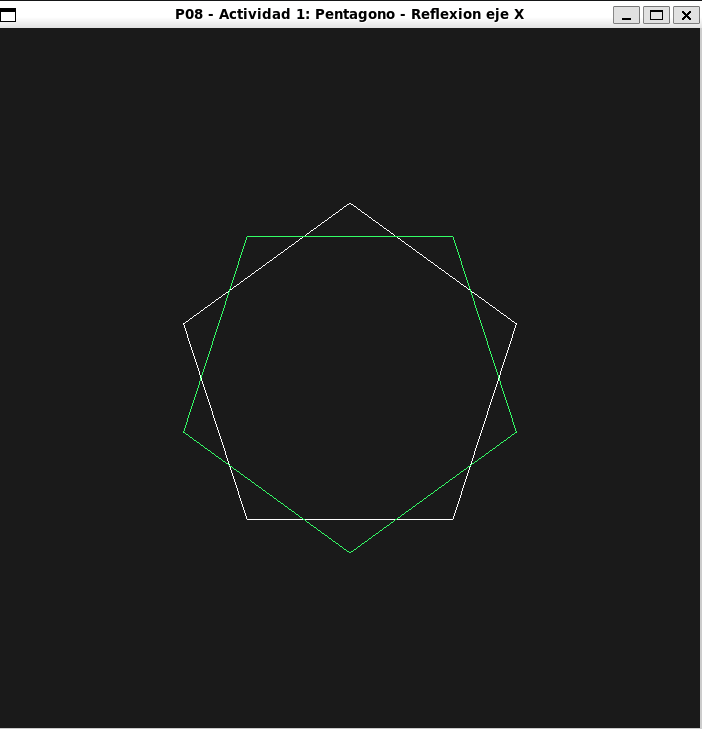
\includegraphics[width=0.8\linewidth]{reflexion pentagono.png}
	\caption{Pent\'agono original y reflejado en el eje X.}
\end{figure}

\begin{lstlisting}[style=cxx,caption={Fragmento principal del ejercicio del pent\'agono.}]
configureGlfwForX11();
if (!glfwInit()) {
	std::cerr << "Error al inicializar GLFW" << std::endl;
	return -1;
}

float finalReflectXMatrix[16];
createScaleMatrix(finalReflectXMatrix, 1.0f, -1.0f);
glUniformMatrix4fv(transformLoc, 1, GL_FALSE, finalReflectXMatrix);
glDrawArrays(GL_LINE_LOOP, 0, N);
\end{lstlisting}

\section*{Ejercicio 2: Reflexi\'on general del tri\'angulo}
El programa \texttt{actividadTriangulo} refleja un tri\'angulo respecto a una recta que pasa por el origen. En esta pr\'actica se us\'o la recta $Y=X$, equivalente a $\theta=45^\circ$.

\[
M(\theta)=R(\theta)\,R_x\,R(-\theta)
\]

\begin{figure}[H]
	\centering
	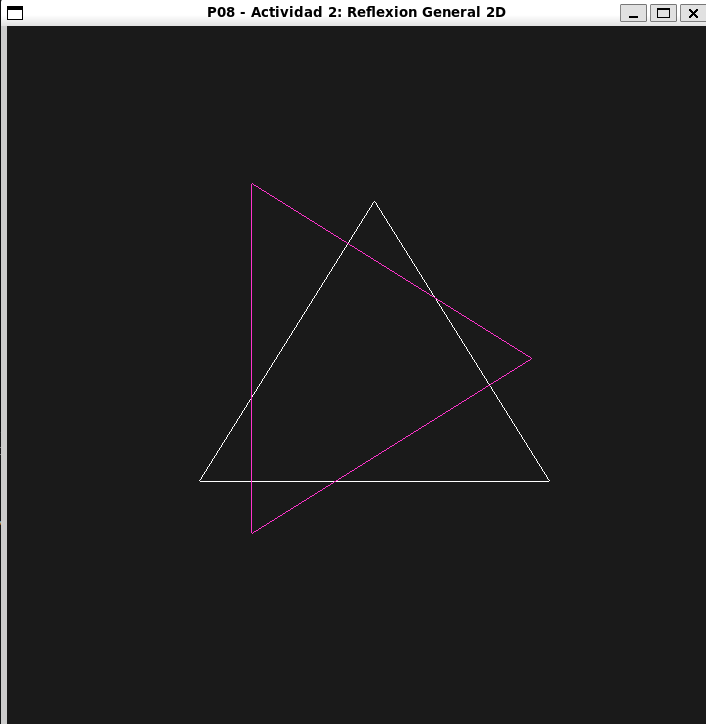
\includegraphics[width=0.8\linewidth]{reflexion triangulo.png}
	\caption{Tri\'angulo original y reflexi\'on general respecto a $Y=X$.}
\end{figure}

\begin{lstlisting}[style=cxx,caption={Construcci\'on de la reflexi\'on general.}]
void reflexionGeneral(float* result, float theta)
{
	float Rpos[16], RefX[16], Rneg[16], tmp[16];
	createRotationMatrix(Rpos, theta);
	createScaleMatrix(RefX, 1.0f, -1.0f);
	createRotationMatrix(Rneg, -theta);
	multiplyMatrices(RefX, Rneg, tmp);
	multiplyMatrices(Rpos, tmp, result);
}
\end{lstlisting}

\section*{Ejemplo del PDF: Transformaciones 2D}
El archivo \texttt{reflexion} reproduce el ejemplo del PDF con escalamiento respecto a un punto fijo y reflexi\'on respecto a los ejes X e Y.

\begin{figure}[H]
	\centering
	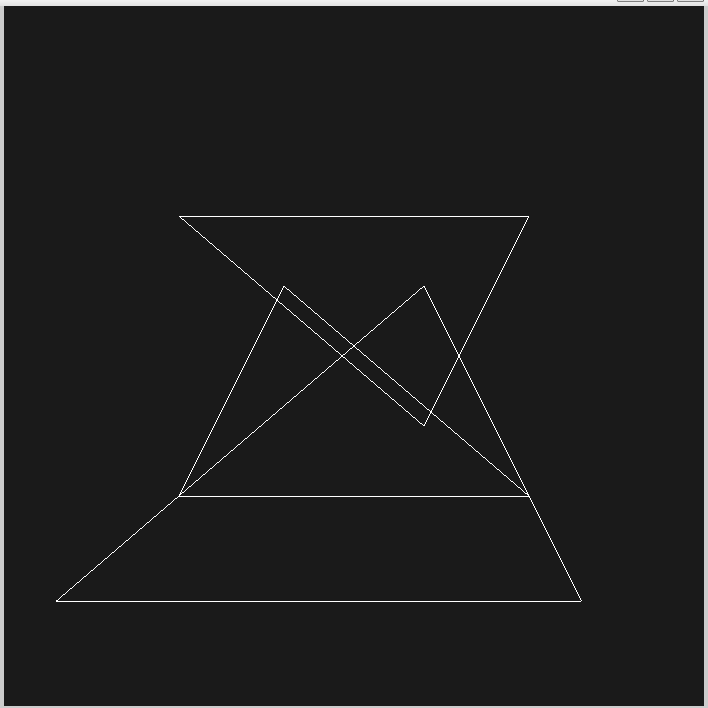
\includegraphics[width=0.8\linewidth]{reflexion 2d.png}
	\caption{Ejemplo del PDF con triangulo original, escalado y reflexiones.}
\end{figure}

\begin{lstlisting}[style=cxx,caption={Helpers comunes movidos a un archivo compartido.}]
inline void createScaleMatrix(float* mat, float sx, float sy)
{
	createIdentityMatrix(mat);
	mat[0] = sx;
	mat[5] = sy;
}

inline void configureGlfwForX11()
{
	glfwInitHint(GLFW_PLATFORM, GLFW_PLATFORM_X11);
}
\end{lstlisting}

\section*{Limpieza de c\'odigo}
Para mejorar la mantenibilidad se centralizaron utilidades compartidas en \texttt{src/gl\_common.hpp}. Con ello se evit\'o repetir c\'odigo para matrices, rotaciones, escalamiento, inicializaci\'on de GLFW y compilaci\'on de shaders.

\begin{itemize}
	\item Se unific\'o la configuraci\'on de GLFW para WSL con X11.
	\item Se centralizaron las funciones matem\'aticas 2D en un solo encabezado.
	\item Se simplific\'o la inicializaci\'on de shaders con una rutina com\'un.
	\item Se retiraron mensajes de depuraci\'on temporales del ejecutable.
\end{itemize}

\section*{Conclusiones}
Se comprob\'o que las reflexiones 2D pueden implementarse con matrices homog\'eneas de manera directa y ordenada. Adem\'as, la refactorizaci\'on realizada permiti\'o que los tres programas compartan c\'odigo com\'un sin afectar su funcionamiento.

\end{document}
